% options:
% thesis=B bachelor's thesis
% thesis=M master's thesis
% czech thesis in Czech language
% english thesis in English language
% hidelinks remove colour boxes around hyperlinks

\documentclass[thesis=B,english]{FITthesis}[2012/10/20]

% \usepackage[utf8]{inputenc} % LaTeX source encoded as UTF-8
% \usepackage[latin2]{inputenc} % LaTeX source encoded as ISO-8859-2
% \usepackage[cp1250]{inputenc} % LaTeX source encoded as Windows-1250

\usepackage{graphicx} %graphics files inclusion
% \usepackage{subfig} %subfigures
% \usepackage{amsmath} %advanced maths
% \usepackage{amssymb} %additional math symbols

\usepackage{dirtree} %directory tree visualisation

% % list of acronyms
% \usepackage[acronym,nonumberlist,toc,numberedsection=autolabel]{glossaries}
% \iflanguage{czech}{\renewcommand*{\acronymname}{Seznam pou{\v z}it{\' y}ch zkratek}}{}
% \makeglossaries

% % % % % % % % % % % % % % % % % % % % % % % % % % % % % % 
% EDIT THIS
% % % % % % % % % % % % % % % % % % % % % % % % % % % % % % 
\setcounter{tocdepth}{2}
\department{Department of Software Engineering}
\title{Adobe Premiere Pro Plugin for NARRA}
\authorGN{Dmitry} %author's given name/names
\authorFN{Vanyagin} %author's surname
\author{Dmitry Vanyagin} %author's name without academic degrees
\authorWithDegrees{Dmitry Vanyagin} %author's name with academic degrees
\supervisor{Petr Pulc}
\acknowledgements{THANKS}
\abstractEN{Summarize the contents and contribution of your work in a few sentences in English language.}
\abstractCS{V n{\v e}kolika v{\v e}t{\' a}ch shr{\v n}te obsah a p{\v r}{\' i}nos t{\' e}to pr{\' a}ce v {\v c}esk{\' e}m jazyce.}
\placeForDeclarationOfAuthenticity{Prague}
\keywordsCS{Replace with comma-separated list of keywords in Czech.}
\keywordsEN{Replace with comma-separated list of keywords in English.}
\declarationOfAuthenticityOption{1} %select as appropriate, according to the desired license

\graphicspath{ {./IMAGES/} }

\begin{document}

% \newacronym{CVUT}{{\v C}VUT}{{\v C}esk{\' e} vysok{\' e} u{\v c}en{\' i} technick{\' e} v Praze}
% \newacronym{FIT}{FIT}{Fakulta informa{\v c}n{\' i}ch technologi{\' i}}

\setsecnumdepth{part}
\chapter{Introduction}
The possibility to visualize and annotate data is always been appreciated in circles of people, who works with a huge amounts of information every day. NARRA is a software that provides this functionality for those using large amounts of video in their practice – artists collaborating on open narratives, video editors, social scientists using video as a research tool, documentary filmmakers with expanded projects. 

Artists can tell stories together using video. Instead of a linear narrative, media works can have multiple paths, multiple versions. The software can be used to create, visualize and navigate a tree of linked stories.

Video editors faced with hundreds of hours of material can annotate their media objects and then organize it based on complex search categories. The software itself will use existing software libraries to add functionality and perform automated annotations. For example the software can extract spoken words and make them into attached text; list shot size, geographic location, etc.

The main purpose of this thesis is to create a tool to use all this functionality and communicate with NARRA directly from your computer. I chose to implement it as a plug-in for Adobe Premiere Pro video editing software application. This application is widely used by different broadcasters such as the BBC\cite{bbc} and CNN\cite{cnn}, also many people chose it as a part or their workflow. Using this plug-in user will be able to directly communicate with NARRA API, i.e., to import and export sequences of clips with all attached metadata. 

To develop this tool I will use mainly Adobe Premiere Pro SDK and Third-party libraries for solving arising problems or for extending functionality provided by SDK.
\chapter{Analysis}
\section{Requirements specification}
\subsection{Functional requirements}
Final product have to fulfill basic requirements:
	\begin{description}
		\item [Authorization in NARRA] 
User should be able to authorize in NARRA, get a token that will be used for all transactions between plug-in and NARRA API. Since Google identities are used inside NARRA, plug-in should communicate with Google authorization services.
		\item [Displaying a list of uploaded projects]
User should be able to browse a list of his projects that he exported to NARRA.
		\item [Searching a project by name]
Plug-in should provide convenient search input field for a user to search in a project list.
		\item [Importing a project from NARRA to Adobe Premiere Pro]
User should be able to choose a project from his project list and import it in the Adobe Premiere Pro.
		\item [Exporting a new project from Adobe Premiere Pro to NARRA]
User should be able to export a new project from Adobe Premiere Pro to NARRA.
		\item [Pushing changes of a project to NARRA]
User should be able to synchronize all changes made in project with NARRA.
		\item [Synchronization of project metadata between NARRA and local machine]
Plug-in should support synchronization of project metadata between NARRA and Adobe Premiere Pro project.
	\end{description}
\subsection{Non-Functional requirements}
	\begin{itemize}
		\item User interface should be clear and understandable for a user.
		\item Plug-in should estimate the length operations and provide a visual representation (progress bars)
		\item Plug-in should work in Adobe Premiere Pro CS5.5 and newer versions.
		\item Internet connection is required to use all functionality.
	\end{itemize}
\section{Use cases}
In this section I will try to describe the basic use cases for this application. In order to communicate with NARRA, user has to complete authorization process, that's why almost every use case require user to be logged in. You can see use case diagram on figure \ref{fig:usecase}.
	\begin{description}
		\item[Authorization in NARRA] 
User wants to authorize himself in order to use plug-in. After plug-in launch, user has to choose an authorization method (choose entity provider). There is two possibilities:
	\begin{itemize}
		\item Authorization using Google account.
		\item Authorization using Github account.
	\end{itemize}
After user clicks on one of these buttons, system default web browser will be launched and user will be redirected to a login page of chosen entity provider. On this page user enters his/her credentials and submits the form. After successful authorization, user's access token will be displayed. This token has to be copied by user to an input field in the plug-in and submitted. 
		\item[Browsing project list] 
User can see a list of his/her projects in NARRA. Requirements: User has to be logged in. There are several way how to access project list:
	\begin{itemize}
		\item After successful authorization, list of projects that given user contributes to will be displayed. 
		\item User can click "Projects" menu button to get to the list of projects from any part of the plug-in.
	\end{itemize}
		\item[Browsing library list] 
User can see a list of his/her libraries in NARRA. Requirements: User has to be logged in. There are several way how to access library list:
	\begin{itemize}
		\item After successful authorization, list of projects that given user contributes to will be displayed, user clicks on the desired project to see which libraries this project contain. List of libraries appears. 
		\item User can click "Libraries" menu button to get to the list of libraries from any part of the plug-in.
	\end{itemize}
		\item[Import new item from NARRA]
User wants to import an item from NARRA. Requirements: User has to be logged in. User navigates to
		\item[Export project to NARRA]
User wants to export a project to NARRA. Current project in Adobe Premiere Pro will be pushed to NARRA after successful launch. User sees progress bar of export process with time estimation. Requirements: User has to be logged in.
		\item[Editing of metadata]
User wants to edit project metadata and save changes back to NARRA. User can add metadata using Adobe Premiere Pro tools. Requirements: User has to be logged in.
		\item[Searching for a project]
User wants to find a project in his project list. Name of the project should be written in a search box. List of projects will be automatically refreshed after each letter typed in search box. Requirements: User has to be logged in.
	\end{description}
	\begin{figure}
		\centering
		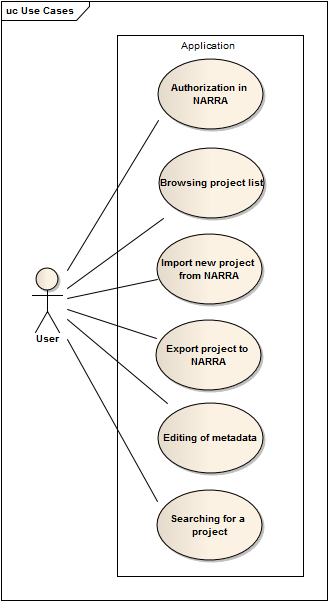
\includegraphics[width=0.7\textwidth]{UseCases.png}
		\caption{Use case diagram}\label{fig:usecase}
	\end{figure}
\section{Structure of application}
I decided to split this application into two plug-ins:
	\begin{itemize}
		\item Import plug-in (Importer).
		\item Export plug-in (Exporter).
	\end{itemize}
The reason why I chose this structure is because it is more logical to have two lightweight plug-ins that solve it's own task. If user wants to import a project into Adobe Premiere Pro, he/she can launch Importer, to export a project Exporter can be used. On figure \ref{fig:narrastruct} you can see a sketch of communication between application and NARRA, you can see that plug-in directly uses Adobe Premiere Pro SDK and communicates with NARRA using http requests. All video files are stored in a cloud storage.
	\begin{figure}
		\centering
		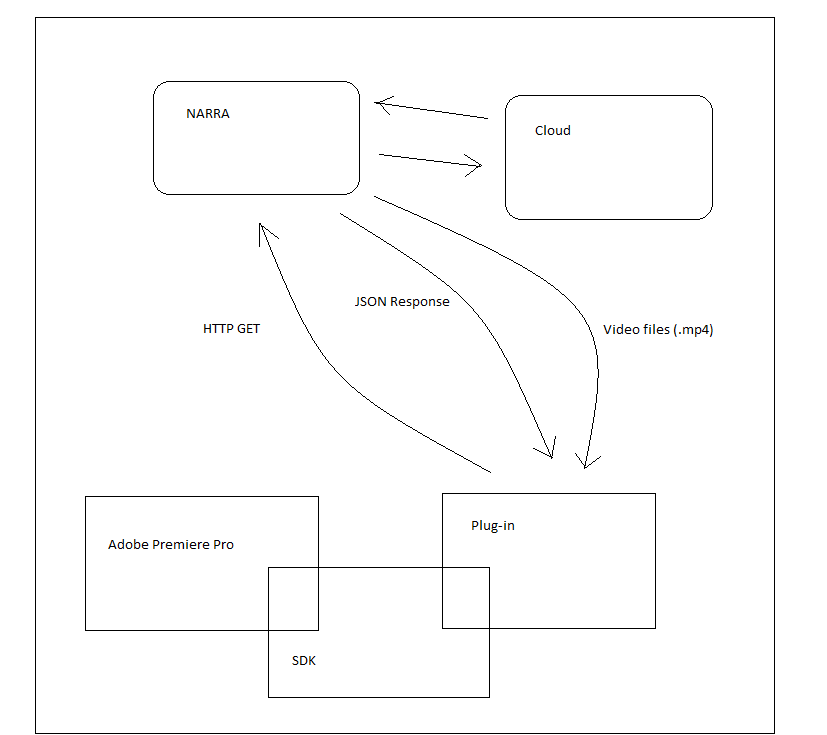
\includegraphics[width=1\textwidth]{StructureofNARRA.png}
		\caption{Sketch of communication with NARRA}\label{fig:narrastruct}
	\end{figure}
\section{Authorization}
To communicate with NARRA, user has to be authorized. NARRA uses Google and Github identities as a user objects, that is the reason why I have to somehow embed authorization service into this plug-in. I decided to do by using a web browser and login form provided by entity providers. Basic scenarion will be like this:
	\begin{enumerate}
		\item User launches plug-in.
		\item User selects authorization method.
		\item Browser window opens up and redirects to Google/Github (depends on the user's choice).
		\item User sees login form.
		\item User enters his/her username and password and allows plug-in to use profile data.
		\item User copies token from browser window and copies it back to NARRA plug-in
	\end{enumerate}
I decided to make user copy token manually because of the built-in browser limitations, it is impossible to create another tab or make a popup, so I have to use default browser for user authorization. I didn't find any way how to pass token from one browser to another, so manual way is the only solution for now.   
\subsection{OAuth 2.0}
OAuth is an open standard for authorization. OAuth provides client applications a "secure delegated access" to server resources on behalf of a resource owner. It specifies a process for resource owners to authorize third-party access to their server resources without sharing their credentials. 

Designed specifically to work with Hypertext Transfer Protocol (HTTP), OAuth essentially allows access tokens to be issued to third-party clients by an authorization server, with the approval of the resource owner, or end-user. The client then uses the access token to access the protected resources hosted by the resource server. OAuth is commonly used as a way for web surfers to log into third party web sites using their Microsoft, Google, Facebook or Twitter accounts, without worrying about their access credentials being compromised.\cite{oauth}

In order to use OAuth 2.0, the installed application must either have access to the system browser, or it must have a browser embedded as a web view. The OAuth 2.0 flow for installed applications is as follows:
	\begin{enumerate}
		\item Your application redirects a browser to a Google URL. The URL query parameters indicate the type of Google API access that the application requires.
		\item As in other scenarios, Google handles user authentication and consent, and the result of the sequence is an authorization code. The authorization code is returned in the title bar of the browser or as a query string parameter, depending on the parameters your application sends in the request.
		\item Your application exchanges the authorization code for an access token and a refresh token. During this exchange, the application presents its client ID and client secret that is obtained from the Developers Console.
		\item Your application uses the access token to make calls to a Google API and stores the refresh token for future use.\cite{oauthdesc}
	\end{enumerate}
As we can see from OAuth web flow (figure \ref{fig:oauth}), authorization process goes in two steps, I need to somehow do it in a way that is convenient for a user. I decided to start this process by pressing a button, request token will be formed automatically and sent to Google. Second task is to figure out how to get authorization code to our application in order to exchange it for an access token later. One way is to make user to enter authorization code to the application (that will be displayed in browser window after user provide his/her credentials and agrees that our plug-in will use profile information), second way is to get this code as part of the query string that is sent to localhost.\cite{oauthdesc}

Parameters that are interesting for us to form request token:
	\begin{description}
		\item[redirect\_uri] 
Determines where the response is sent. The value of this parameter must exactly match one of the values that appear in the Credentials page in the Google Developers Console (including the http or https scheme, case, and trailing slash). You may choose between urn:ietf:wg:oauth:2.0:oob, urn:ietf:wg:oauth:2.0:oob:auto, or an http://localhost port. Value of this parameter will determine the way of getting authorization code that we will exchange for an access token.
		\item[client\_id] 
Identifies the client that is making the request. The value passed in this parameter must exactly match the value shown in the Google Developers Console.
	\end{description}

	\begin{figure}
		\centering
		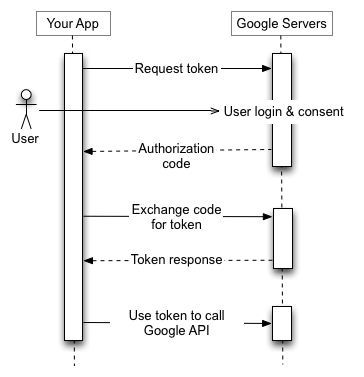
\includegraphics[width=0.7\textwidth]{oauthwebflow.png}
		\caption{OAuth web flow}\label{fig:oauth}
	\end{figure}
\section{Paradigm shift}
At first glance we thought that Creative Suite version of Adobe Premiere Pro with provided SDK will be enough to implement desired functionality of the plug-in, but we encountered a problem with operating multiple files in project bin. There is no possibility to realize correct importing of project files into Adobe Premiere Pro CS5.5, so we decided to completely shift our paradigm and choose different approach to problem solving. We understand that we lose the flexibility of C language and possibility of usage many different frameworks and libraries, but in order to realize our needs it is necessary.
\subsection{Adobe Premiere Pro CC}
Creative Cloud (CC) version of Adobe products is the successor to Creative Suite that we chose as our working environment before encountering a problem. Adobe Premiere Pro CC allows us to use Panel SDK that provides much more functionality in comparison with SDK for Creative Suite version of video editing tool. 

Adobe announced that it will no longer release any products of CS version\cite{CC}, so choosing CC we also looking to the future. 

Adobe Premiere Pro CC 2014 uses built-in web browser for executing plug-ins, so that means that we can use standard tools for web development to implement our plug-in.

\section{ExtendScript}
ExtendScript is a programming language, that is used for scripting Adobe products. We will use it as a layer between our plug-in and Adobe Premiere Pro since it can operate functions of this software directly. It has very similar structure and syntax with JavaScript because both of these programming languages are just different versions of ECMAScript.
\subsection{ECMAScript}
This Ecma Standard is based on several originating technologies, the most well known being JavaScript (Netscape) and JScript (Microsoft). The language was invented by Brendan Eich at Netscape and first appeared in that company’s Navigator 2.0 browser. It has appeared in all subsequent browsers from Netscape and in all browsers from Microsoft starting with Internet Explorer 3.0.

ECMAScript is an object-oriented programming language for performing computations and manipulating computational objects within a host environment. ECMAScript is not intended to be computationally self-sufficient; indeed, there are no provisions in this specification for input of external data or output of computed results. Instead, it is expected that the computational environment of an ECMAScript program will provide not only the objects and other facilities described in this specification but also certain environment-specific host objects, whose description and behaviour are beyond the scope of this specification except to indicate that they may provide certain properties that can be accessed and certain functions that can be called from an ECMAScript program.

A \textbf{scripting language} is a programming language that is used to manipulate, customise, and automate the facilities of an existing system. In such systems, useful functionality is already available through a user interface, and the scripting language is a mechanism for exposing that functionality to program control. In this way, the existing system is said to provide a host environment of objects and facilities, which completes the capabilities of the scripting language. A scripting language is intended for use by both professional and non-professional programmers.

	\begin{itemize}
\item ECMAScript is object-based: basic language and host facilities are provided by objects, and an ECMAScript program is a cluster of communicating objects. An ECMAScript object is a collection of properties each with zero or more attributes that determine how each property can be used - for example, when the Writable attribute for a property is set to false, any attempt by executed ECMAScript code to change the value of the property fails. Properties are containers that hold other objects, primitive values, or functions. A primitive value is a member of one of the following built-in types: Undefined, Null, Boolean, Number, and String; an object is a member of the remaining built-in type Object; and a function is a callable object. A function that is associated with an object via a property is a method.
\item ECMAScript defines a collection of built-in objects that round out the definition of ECMAScript entities. These built-in objects include the global object, the Object object, the Function object, the Array object, the String object, the Boolean object, the Number object, the Math object, the Date object, the RegExp object, the JSON object, and the Error objects Error, EvalError, RangeError, ReferenceError, SyntaxError, TypeError and URIError.
\item ECMAScript also defines a set of built-in operators. ECMAScript operators include various unary operations, multiplicative operators, additive operators, bitwise shift operators, relational operators, equality operators, binary bitwise operators, binary logical operators, assignment operators, and the comma operator.
\item ECMAScript syntax intentionally resembles Java syntax. ECMAScript syntax is relaxed to enable it to serve as an easy-to-use scripting language. For example, a variable is not required to have its type declared nor are types associated with properties, and defined functions are not required to have their declarations appear textually before calls to them.\cite{ecma}
	\end{itemize}

\section{NARRA API}
I this section I would like to describe a layer between our plug-in and NARRA. At first I will analyze different methods of building web API, compare them and then I will write about particular implementation of NARRA API.

\textbf{Application programming interface} (API) is a set of routines, protocols, and tools for building software applications. An API expresses a software component in terms of its operations, inputs, outputs, and underlying types. An API defines functionalities that are independent of their respective implementations, which allows definitions and implementations to vary without compromising each other.

\subsection{SOAP}
SOAP is an XML language defining a message architecture and message formats, hence providing a rudimentary processing protocol. The SOAP document defines a toplevel XML element called envelope, which contains a headerand a body. The SOAP header is an extensible container for message-layer infrastructure information that can be used for routing purposes (e.g., addressing) and Quality of Service (QoS) configuration (e.g., transactions, security, reliability). The body contains the payload of the message. XML Schema is used to describe the structure of the SOAP message, so that SOAP engines at the two endpoints can marshall and unmarshall the message content and route it to the appropriate implementation.

\textbf{Web Services Description Language} (WSDL) is an XML language for defining interfaces syntactically. A WSDL port type contains multiple abstract operations, which are associated with some incoming and outgoing messages. The WSDL binding links the set of abstract operations with concrete transport protocols and serialization formats. By default, there is no notion of state. The interaction with stateful Web services is covered by the WS-Resource Framework, which handles the management of stateful resources behind a Web service interface.

	\begin{description}
		\item[Strength of SOAP] 
SOAP message format and the WSDL interface definition language have gained popularity as the technologies capable of delivering interoperability between systems. One advantage is protocol transparency and independence.

Using SOAP, the same message in the same format can be transported across a variety of  systems, which may rely on HTTP, but also on many other transports. The transport protocol may change along the way.

Using WSDL to describe a service interface helps to abstract from the underlying communication protocol and serialization details as well as from the service implementation platform (operating system and programming language). WSDL contracts provide a machine-processable description of the syntax and structure of the corresponding request and response messages and define a flexible evolution path for the service. 

As business and technology requirements change, the same abstract service interface can be bound to different transport protocols and messaging endpoints. In particular, WSDL can model service interfaces for systems based on synchronous and asynchronous interaction patterns.\cite{soaprest}
		\item[Weaknesses of SOAP] 
Paradoxically, the power of SOAP can also be misused. Thus, it is important to avoid leakage across abstraction levels. Interoperability problems can occur when, for instance, native data types and language constructs of the service implementation are present in its interface.\cite{soaprest}

The translation between the XML and the corresponding memory data structures has been problematic and is the main source of performance inefficiencies. Furthermore, XML Schema is a very rich language, making it difficult to identify the right construct to express a data model in a way that is fully supported by all SOAP/WSDL implementations.\cite{soaprest}
	\end{description}
\subsection{REST}
REpresentational State Transfer (REST) was originally introduced as an architectural style for building large-scale distributed hypermedia systems.

The REST architectural style is based on four principles:
	\begin{description}
		\item[Resource identification through URI.] A RESTful Web service exposes a set of resources which identify the targets of the interaction with its clients. Resources are identified by URIs, which provide a global addressing space for resource and service discovery. 			\item[Uniform interface.] Resources are manipulated using a fixed set of four create, read, update, delete operations: PUT, GET, POST, and DELETE. PUT creates a new resource, which can be then deleted using DELETE. GET retrieves the current state of a resource in some representation. POST transfers a new state onto a resource.\cite{soaprest}
		\item[Self-descriptive messages.] Resources are decoupled from their representation so that their content can be accessed in a variety of formats (e.g., HTML, XML, plain text, PDF, JPEG, etc.). Metadata about the resource is available and used, for example, to control caching, detect transmission errors, negotiate the appropriate representation format, and perform authentication or access control. 
		\item[Stateful interactions through hyperlinks.] Every interaction with a resource is stateless, i.e., request messages are self-contained. Stateful interactions are based on the concept of explicit state transfer. Several techniques exist to exchange state, e.g., URI rewriting, cookies, and hidden form fields. State can be embedded in response messages to point to valid future states of the interaction.\cite{soaprest}
	\end{description}
Now I want to describe strengths and weaknesses of REST:
	\begin{description}
		\item[Strength of REST] 
RESTful Web services are designed to be simple. HTTP clients and servers are available for all major programming languages and operating system/hardware platforms, and the default HTTP port 80 is commonly left open by default in most firewall configurations. Such lightweight infrastructure, is inexpensive to acquire and thus has a very low barrier for adoption.

The effort required to build a client to a RESTful service is very small as developers can begin testing such services from an ordinary Web browser, without having to develop custom client-side software.\cite{soaprest} 

Deploying a RESTful Web service is very similar to building a dynamic Web site. Furthermore, thanks to URIs and hyperlinks, REST has shown that it is possible to discover Web resources without an approach based on compulsory registration to a (centralized) repository. On the operational side, it is known how to scale a stateless RESTful Web service to serve a very large number of clients, thanks to the support for caching, clustering and load balancing built into REST. Due to the possibility of choosing lightweight message formats, e.g., the JavaScript Object Notation (JSON) or, even plain text for very simple data types, REST also gives more possibilities to optimize the performance of a Web service.
		\item[Weaknesses of REST] 
There is some confusion regarding the commonly accepted best practices for building RESTful Web services. Recommendations have been established informally. 

Most of the REST services uses just GET and POST (first for idempotent requests, second for everything else) because some proxies and firewalls may not always allow connections that use other method.
These restrictions have led to a series of workarounds, where the "real" verb is sent using either a special HTTP header (X-HTTP-Method-Override). As with most non-standard workarounds, these may not be understood by all Web servers, and require additional development and testing effort. Another limitation makes it impossible to strictly follow the GET vs. POST rule. For idempotent requests having large amounts of input data (more than 4 KB in most current implementations) it is not possible to encode such data in the resource URI, as the server will reject such URI or in the worst case it will crash, exposing the service to buffer overflow attacks. The size of the request notwithstanding, it may also be challenging to encode complex data structures into a URI as there is no commonly accepted marshalling mechanism. Inherently, the POST method does not suffer from such limitations.\cite{soaprest}
	\end{description}
\chapter{Design}
\chapter{Adobe Premiere Pro}
\section{Overview}

Adobe Premiere Pro is a timeline-based video editing software application. It is part of the Adobe Creative Cloud, which includes video editing, graphic design, and web development programs.

Premiere Pro has been used to edit feature films, such as Gone Girl, Captain Abu Raed, and Monsters, and other venues such as Madonna's Confessions Tour.\cite{adobe}

	\begin{figure}
		\centering
		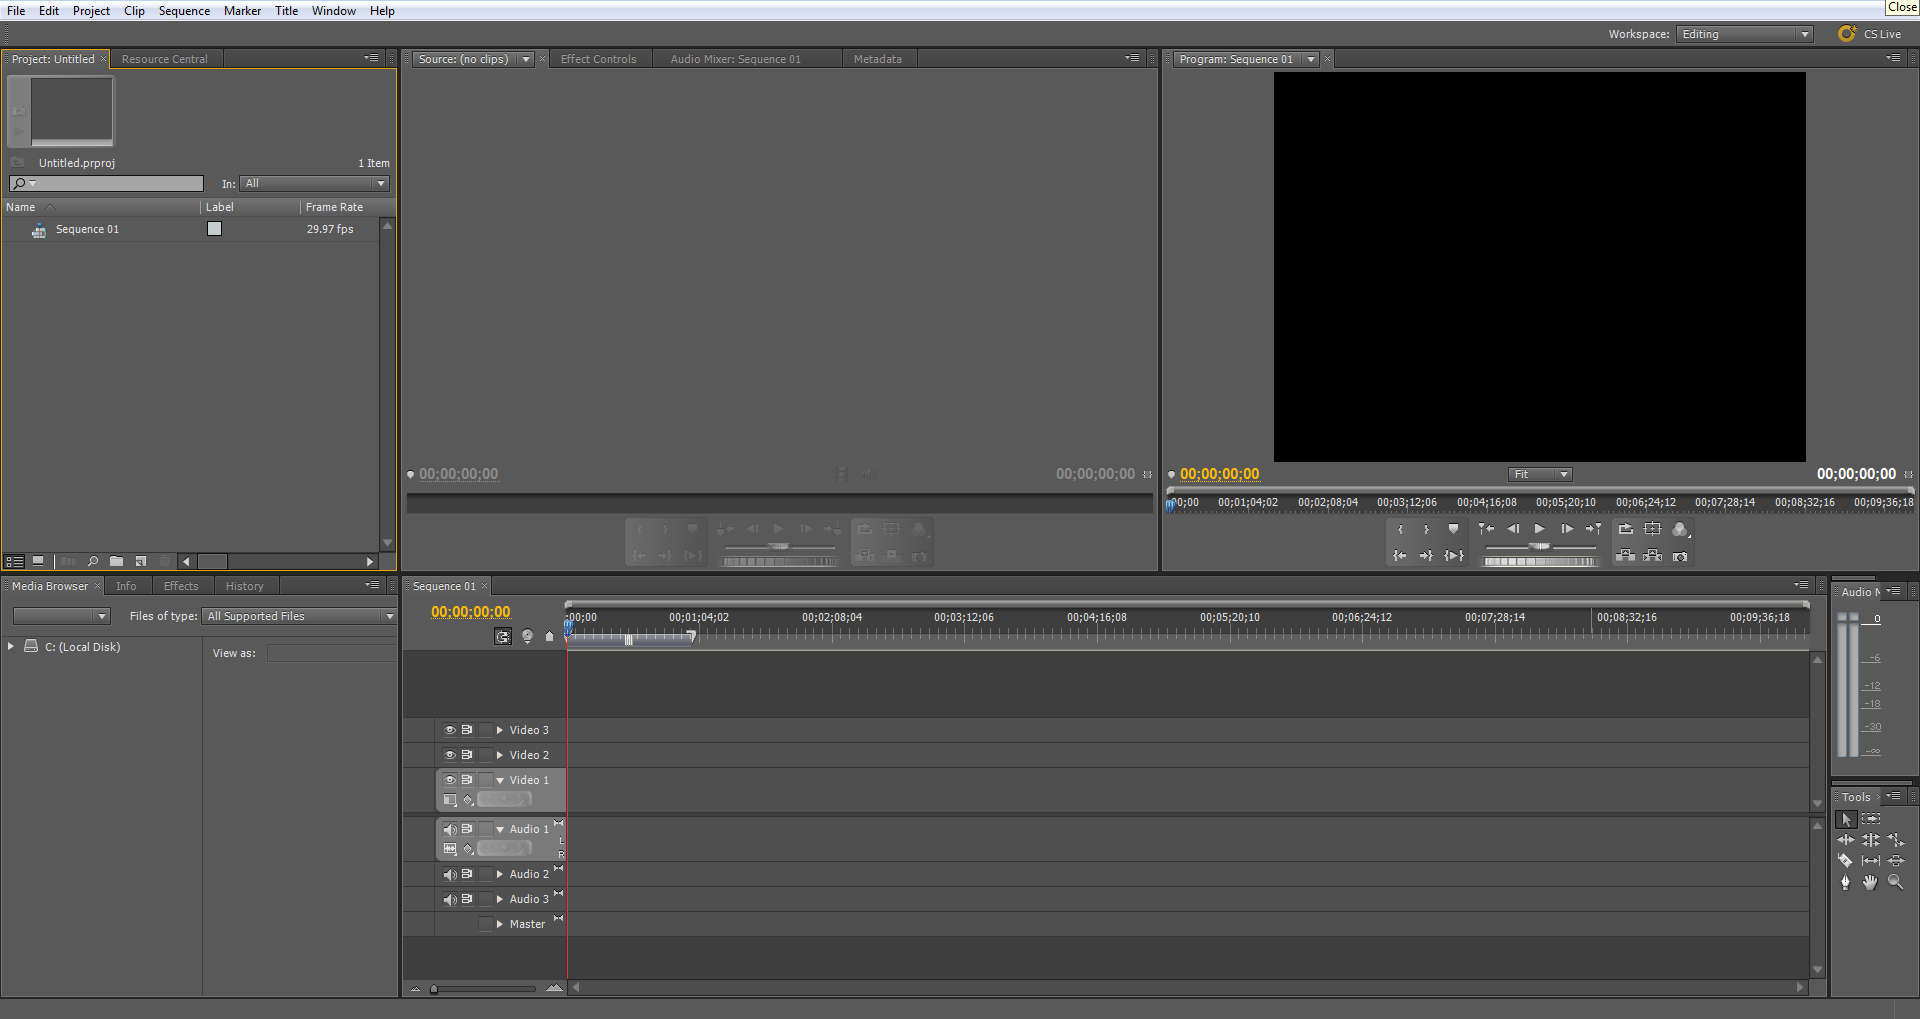
\includegraphics[width=0.8\textwidth]{PremiereMain.png}
		\caption{Adobe Premiere Pro CS5.5 window}\label{fig:APPWindow}
	\end{figure}

\section{History}

Premiere Pro is the redesigned successor to Adobe Premiere, and was launched in 2003. Premiere Pro refers to versions released in 2003 and later, whereas Premiere refers to the earlier releases. Premiere was one of the first computer-based NLEs (non-linear editing system), with its first release on Mac in 1991. Up until version Premiere Pro 2.0 (CS2), the software packaging featured a galloping horse, in a nod to Eadweard Muybridge's work, "Sallie Gardner at a Gallop".\cite{adobe}

\chapter{Implementation}

\setsecnumdepth{part}
\chapter{Conclusion}


\bibliographystyle{iso690}
\bibliography{Bibliography}

\setsecnumdepth{all}
\appendix

\chapter{Acronyms}
% \printglossaries
\begin{description}
	\item[GUI] Graphical user interface
	\item[XML] Extensible markup language
\end{description}


\chapter{Contents of enclosed CD}

%change appropriately

\begin{figure}
	\dirtree{%
		.1 readme.txt\DTcomment{the file with CD contents description}.
		.1 exe\DTcomment{the directory with executables}.
		.1 src\DTcomment{the directory of source codes}.
		.2 wbdcm\DTcomment{implementation sources}.
		.2 thesis\DTcomment{the directory of \LaTeX{} source codes of the thesis}.
		.1 text\DTcomment{the thesis text directory}.
		.2 thesis.pdf\DTcomment{the thesis text in PDF format}.
		.2 thesis.ps\DTcomment{the thesis text in PS format}.
	}
\end{figure}

\end{document}
